\documentclass[]{article}
\usepackage{amsmath,amssymb,amsfonts,amsbsy}
\usepackage{indentfirst}
\usepackage{fancybox}
\usepackage{graphicx}
\usepackage{soul,soulutf8}
\usepackage{url,color}
\usepackage{fullpage}
\usepackage{tikz}
\usepackage{float}
\usepackage{subcaption}
\usepackage{wrapfig}


\usetikzlibrary{shapes, arrows}

\usepackage[autocite=footnote,
    backend=bibtex,
    citestyle=ieee,
    isbn=false,
    doi=false,
    url=false
]{biblatex}
\addbibresource{IT.bib}


%\baselineskip=15pt
% \pagestyle{plain}   %with page numbers
% \pagestyle{empty} %without page numbers

\renewcommand{\baselinestretch}{1.25}
\newcommand{\R}{\mathbb{R}}
\newcommand{\cX}{\mathcal{X}}
%\newcommand{\tr}{\mathrm{tr}}
\renewcommand{\st}{\mathrm{s.t.}}

% Define block styles
\tikzstyle{decision} = [diamond, draw, fill=blue!20, 
text width=4.5em, text badly centered, node distance=3cm, inner sep=0pt]
\tikzstyle{block} = [rectangle, draw, fill=blue!20, 
text width=6em, text centered, rounded corners, minimum height=4em, minimum width=8em, scale=.6]

\tikzstyle{blockq} = [rectangle, draw, fill=red!20, 
text width=6em, text centered, rounded corners, minimum height=4em, minimum width=8em, scale=.6]

\tikzstyle{line} = [draw, -latex']
\tikzstyle{cloud} = [draw, ellipse,fill=red!20, node distance=3cm,
minimum height=2em]

%\usepackage[toc]{multitoc}\begin{minipage}{.6\textwidth}


\begin{document}

%Enter your title here
\title{Profile-Guided Source Coding in Dual-Compilation}
%Enter your name Here
\author{Chenhao Wu}
\date{March, 2019}

\makeatletter
\let\inserttitle\@title
\let\insertauthor\@author
\makeatother

\begin{titlepage}
\centering
{   \textsc{\Large CIE 6020 Information Theory (Spring, 2018)}\\[0.5 cm]}
{\Large\bf Course Project: \inserttitle}\\[.2in]
Name: \underline{\quad\quad \insertauthor \quad\quad  
}
\hspace{0.3in}
ID Number: \underline{\quad\quad
%Enter Your ID number Here
117010285
\quad\quad}
\vspace{0.5 cm}\\
\fbox{\parbox{\textwidth}{
\begin{itemize}
% \item 
% Date assigned: Friday 19/1/2018
% \item 
% Date due: Thursday 1/2/2018, 11:55 PM
\item
This cover sheet must be signed and submitted along with the report on additional sheets
\item
By submitting this report with my name affixed above,
\begin{itemize}
%\item
%I understand that report submitted at 11:56 PM or later will not be accepted,
\item
I acknowledge that I am aware of the University policy concerning academic misconduct (appended below),
\item
I attest that the work I am submitting for this assignment is solely my own, and
\item
I understand that suspiciously similar homework submitted by multiple
individuals will be reported to School and Registry for investigation.
\end{itemize}
\item
Academic Misconduct in any form is in violation of CUHK(SZ)'s Student Disciplinary Regulations and will not be tolerated. This includes, but is not limited to: copying or sharing answers on tests or assignments, plagiarism, having someone else do your academic work or working with someone on homework when not permitted to do so by the instructor. Depending on the act, a student could receive an F grade on the test/assignment, F grade for the course, and could be suspended or expelled from the University.
\end{itemize}}}
\end{titlepage}

%%% Begin of the report 
\maketitle

%\begin{abstract}
%Within this decade, the computing performance of mobiles and embedded systems have been significantly raised such that more computing workloads can be undertaken on mobiles and embedded systems, such as digital image processing, augmented-reality applications, and so on. In practice, one of the critical bottlenecks in mobiles and embedded systems design and optimization is the run-time memory space and power consumption. Since the complexity of program and data set grew much faster than the performance of memory capacity in the mobile and embedded system, rather than merely use expensive computing components to feed the needs of applications with high computing overhead, it is more promising to find ways to best utilize the system use of memory space. To realize this objective, we proposed a profile-guided source coding (PGSC), which will perform an adaptive compiler-guided data compression on memory space during run-time according to different applications and run-time environment.
%\end{abstract}

\section{Introduction}
Within this decade, the computing performance of mobiles and embedded systems have been significantly raised such that more computing workloads can be undertaken on mobiles and embedded systems, such as digital image processing, machine learning and deep learning applications, augmented-reality applications, and so on. In practice, one of the critical bottlenecks in mobiles and embedded systems design and optimization is the run-time memory space and power consumption. Since the complexity of program and data set grew much faster than the performance of memory capacity in the mobile and embedded system, rather than merely use expensive computing components to feed the needs of applications with high computing overhead, it is more promising to find ways to best utilize the system use of memory space. To realize this objective, we proposed a profile-guided source coding (PGSC), which will perform an adaptive compiler-guided data compression on memory space during run-time according to different applications and run-time environment. \par 

\begin{figure}[H]
\begin{minipage}[b][8cm][s]{.27\textwidth}
	\centering
	\vfill
	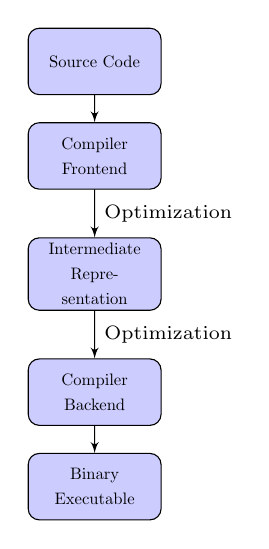
\begin{tikzpicture}[node distance = 2cm, auto]
	
	% Place nodes
	\node [block] 								(Source Code) 					{Source Code};
	\node [block, below of=Source Code] 		(Compiler Frontend)  			{Compiler Frontend};
	\node [block, below of=Compiler Frontend, yshift=-0.5cm] (IR)				{Intermediate Representation};
	\node [block, below of=IR, yshift=-0.5cm]	(Compiler Backend)				{Compiler Backend};
	\node [block, below of=Compiler Backend]	(Binary Executable)				{Binary Executable};
	
	%Draw edges
	\path [line] (Source Code) 		    -- 										(Compiler Frontend);
	\path [line] (Compiler Frontend)    -- node {\scriptsize Optimization} 		(IR);
	\path [line] (IR) 					-- node {\scriptsize Optimization} 		(Compiler Backend);
	\path [line] (Compiler Backend)		--										(Binary Executable);
	
	\end{tikzpicture}
	
	\vfill
	\captionsetup{justification=centering}
	\caption{Traditional Compilation Procedure}
	\label{fig:compil}
	
	\vspace{\baselineskip}
\end{minipage}\qquad
\begin{minipage}[b][8cm][s]{.35\textwidth}
	\centering
	\vfill
	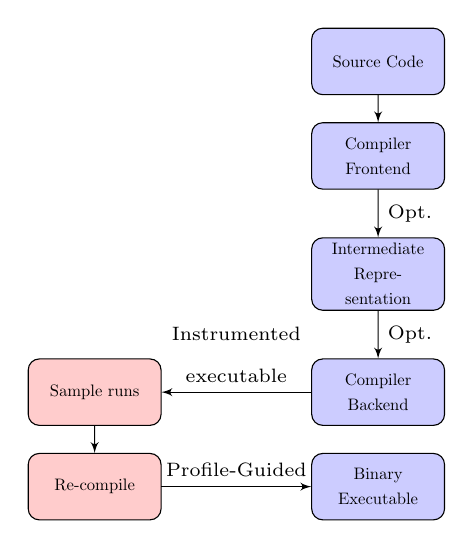
\begin{tikzpicture}[node distance = 2cm, auto]
	
	% Place nodes
	\node [block] 								(Source Code) 					{Source Code};
	\node [block, below of=Source Code] 		(Compiler Frontend)  			{Compiler Frontend};
	\node [block, below of=Compiler Frontend, yshift=-0.5cm] (IR)				{Intermediate Representation};
	\node [block, below of=IR, yshift=-0.5cm]	(Compiler Backend)				{Compiler Backend};
	\node [block, below of=Compiler Backend]	(Binary Executable)				{Binary Executable};
	\node [blockq, left of=Compiler Backend, xshift=-4cm] (SR)				{Sample runs};
	\node [blockq, left of=Binary Executable, xshift=-4cm] (Re-Compile)		{Re-compile};
	
	%Draw edges
	\path [line] (Source Code) 		    -- 										(Compiler Frontend);
	\path [line] (Compiler Frontend)    -- node {\scriptsize Opt.} 		(IR);
	\path [line] (IR) 					-- node {\scriptsize Opt.} 		(Compiler Backend);
	\path [line] (Compiler Backend)		-- node[above, align=center] {\scriptsize Instrumented\\ \scriptsize executable} (SR);
	\path [line] (SR)					-- 									    (Re-Compile);
	\path [line] (Re-Compile)			-- node {\scriptsize Profile-Guided}	(Binary Executable);
	
	\end{tikzpicture}
	\vfill
	\captionsetup{justification=centering}
	\caption{Compilation Procedure with PGO}
	\label{fig:compilpgo}
\end{minipage}\qquad
\begin{minipage}[b][8cm][s]{.3\textwidth}
	\centering
	\vfill
	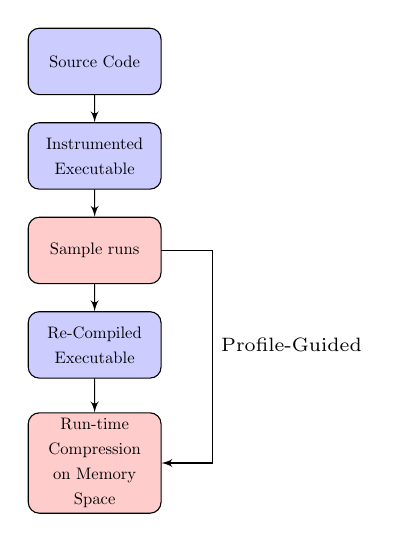
\begin{tikzpicture}[node distance = 2cm, auto]
	
	% Place nodes
	\node [block] 								(Source Code) 					{Source Code};
	\node [block, below of=Source Code] 		(IE) 					 		{Instrumented Executable};
	\node [blockq, below of=IE] 				(SR)							{Sample runs};
	\node [block, below of=SR] 					(Re-Compiled Executable)		{Re-Compiled Executable};
	\node [blockq, below of=Re-Compiled Executable, yshift=-0.5cm] (RC)							{Run-time Compression on Memory Space};	
	\node [label, right of=Re-Compiled Executable, xshift=0.5cm]								(PF)							{\scriptsize Profile-Guided};
	
	%Draw edges
	\path [line] (Source Code) 		    -- 										(IE);
	\path [line] (IE) 					-- 										(SR);
	\path [line] (SR)					--									 	(Re-Compiled Executable);
	\path [line] (Re-Compiled Executable) --									(RC);
	\path [line] (SR)					--++ (1.5, 0)  |-						(RC);
	
	\end{tikzpicture}
	\vfill
	\caption{Profile-Guided Source Coding}
	\captionsetup{justification=centering}
	\label{fig:compilpgosrc}
\end{minipage}
\end{figure}

The idea of this approach comes from a modern compilation technique, Profiled-Guided Optimization (PGO), that as shown in Figure 1 and Figure 2, differed from the traditional approach \cite{CompilerDesign}, the compiler will perform a recompilation based on initial executable and sample runs. A profile, for instance, breaks the source code into blocks and devises a table of the frequency each block is executed via sample runs, and during recompilation, code blocks will be reordered with respect to the frequency table. For example, blocks with higher frequency will be allocated in memory area with lower memory address and blocks with lower frequency will be allocated in higher address so that the additional I/O overhead consumed in function callbacks will be reduced. Similar to previous compiler optimization methods, like the deletion of unreachable code, the constant folding optimization and propagation optimization, the objective of PGO is to further reduce the redundancy of unnecessary and/or unimportant logic branches in the source program. \par 
The usage of this approach, however, can be extended into attempts in reducing the memory space, that after sample runs, not only the frequency of code blocks can be collected, but also the preliminary investigation of frequency that each block of memory is accessed can be gathered as well. As shown in Figure 3, the procedure of PGSC consists of a dual-stage compilation, that the compiler will initially compile the source code into an instrumented executable, and based on a profile generated after sample runs, the compiler will re-compile the source code such that during the run-time, the program will compress specific areas of memory space in order to reduce the redundancy of memory use, and will instantaneously decompress the compressed contents whenever the program needs. \par 
In the tide that more and more applications on mobile and embedded systems behave to buffer long arrays of audio, images and video frames into the memory space during run-time, that in a low frequency the program access to them but they still need to be remained in the memory space, such as intermediate training matrices, sample sets of images and so on, PGSC can regularly compress them to reduce the buffer size. The compression is compiler-guided, thus it can be performed no matter which optimization has been applied onto the program and what third-party library the program has imported. \par 
In this report we will briefly introduce the control flow of PGSC, and methodologies we applied to perform the compression over memory space, and the implementation of a compiler with PGSC. 

\section{Related Work}
\cite{MSAli2008} \cite{OO2009} \cite{KSKO2017} \cite{MTK2011}	
	
%\section{Implementation}

	%\subsection{Compression Method}
	
	%\subsection{Run-time Compression}

\printbibliography


\end{document}
